\section{Results and Analysis}
This section presents the results of the experiments conducted to evaluate the performance of the sequential encounter encoding and the direct encoding in solving the optimization problem.
Because the number of variables and clauses in the CNF encoding when using standard method is too large, we benchmarked the performance of the two encoding methods on a smaller generated dataset.

\subsection{Comparison of Sequential Encounter Encoding and Standard Encoding}

The dataset was generated using the \texttt{input/generate.py} script, which is included in the source code repository.
It is stored in the \texttt{input} directory in the repository.
The dataset used in the experiments was generated using the following parameters:
\begin{itemize}
    \item Number of items: 8
    \item Number of transactions: 28
\end{itemize}

After generating the dataset, the optimization problem was encoded into CNF format using the sequential encounter encoding and the standard encoding.
With timeout 900ms and 1GB memory limit, we ran the Kissat SAT Solver on the CNF file to find all solutions.
The number of clauses and variables in the CNF encoding for each encoding method is shown in Figure \ref{fig:4_1} when Minimum Support is increased from 0.1 to 0.9 (10\% to 90\% of the total transactions).

% figure
\begin{figure}[H]
    \centering
    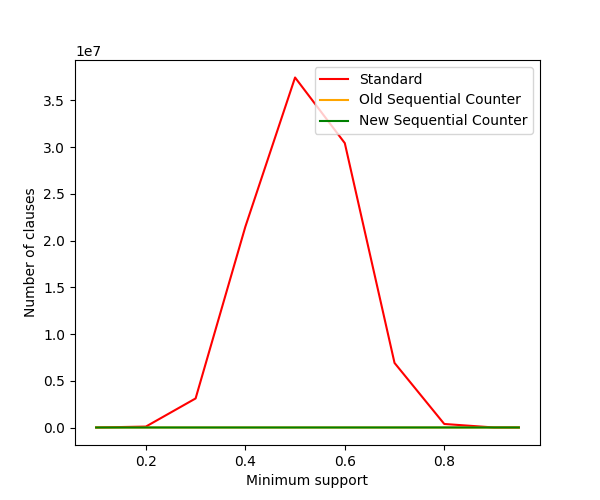
\includegraphics[width=1\textwidth]{chapter4/image/n_trans_28_clauses.png}
    \caption{Comparison of the number of clauses in the CNF encoding of the optimization problem using the sequential encounter encoding and the standard encoding.}
    \label{fig:4_1}
\end{figure}

This graph illustrates a notable difference between the number of clauses in the CNF encoding
utilizing the sequential encounter encoding compared to the standard encoding method. Particularly, it demonstrates that the sequential encounter encoding results in a significantly smaller number of clauses and variables.

Of special interest is the observation that the number of clauses generated by the standard encoding reaches a peak value,
approximately 35 million clauses, as the minimum support approaches the midpoint threshold.
This suggests a critical point where the standard encoding method generates an overwhelming number of clauses,
highlighting the potential inefficiency and scalability issues associated with this approach.

Additionally, the number of clauses generated by the sequential encounter encoding method appears to remain consistently low,
maintaining stability across various levels of minimum support.
This suggests that the sequential encounter encoding method is capable of producing fewer clauses while still ensuring the efficiency of the encoding process,
thus keeping the data analysis process manageable even as the constraints grow larger.

In addition to comparing the number of clauses, we also compared the time taken to find all solutions using both methods.
The results are shown in Figure \ref{fig:4_2}.
% figure
\begin{figure}[H]
    \centering
    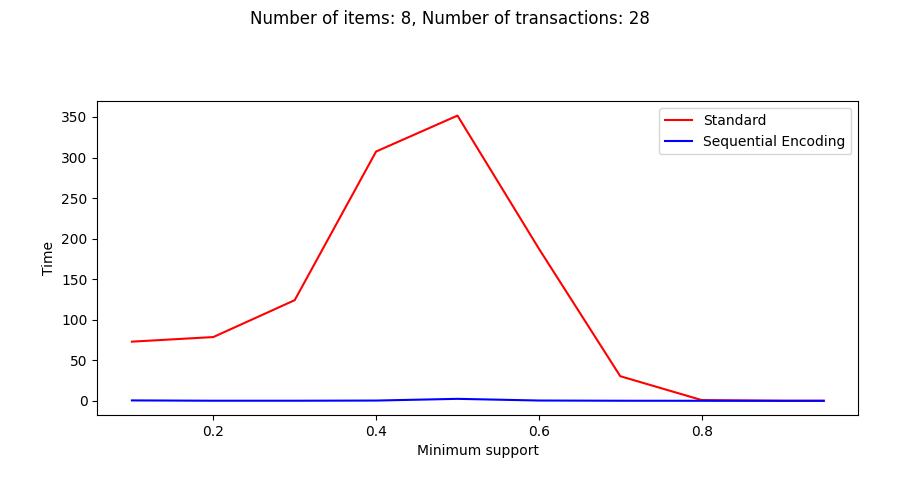
\includegraphics[width=1\textwidth]{chapter4/image/n_trans_28_time.png}
    \caption{Comparison of the time taken to find all solutions using the sequential encounter encoding and the standard encoding}
    \label{fig:4_2}
\end{figure}

The graph indicates that the sequential encounter encoding method consistently outperforms the standard encoding method in terms of time efficiency.
Even as the complexity of the problem increases, the sequential encounter encoding method demonstrates faster solution-finding times,
highlighting its superiority not only in minimizing the number of clauses but also in accelerating the solution discovery process.

However, it's worth noting that while the number of variables may increase, this increment is negligible compared to the significant reduction in the number of clauses.
\begin{figure}[H]
    \centering
    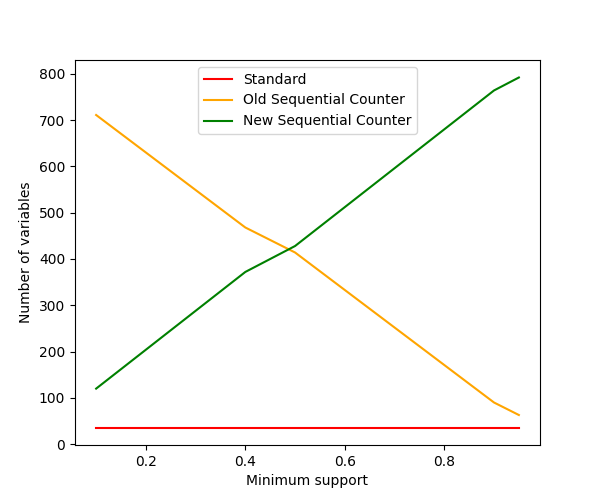
\includegraphics[width=1\textwidth]{chapter4/image/n_trans_28_vars.png}
    \caption{Comparison of the number of variables in the CNF encoding of the optimization problem using the sequential encounter encoding and the standard encoding.}
    \label{fig:4_3}
\end{figure}

This observation underscores the efficiency of the sequential encounter encoding method in striking a balance between the complexity of the problem and the computational resources required.
Despite the slight increase in variables, the overall computational overhead remains substantially lower,
making the sequential encounter encoding method a promising approach for tackling large-scale constraint satisfaction problems.

In addition, the experiments were conducted using various combinations of parameters to evaluate the performance of the sequential encounter encoding and the standard encoding in solving the optimization problem. By varying the number of transactions from 26 to 28 and the minimum support from 0.1 to 0.9, we aimed to assess the scalability and efficiency of both encoding methods across different problem sizes and constraints.
\begin{itemize}
    \item Number of items: 8
    \item Number of transactions: 26 to 28
    \item Minimum Support: 0.1 to 0.9
\end{itemize}

Table \ref{tab:4_1} presents the results obtained from these experiments.
It provides a comprehensive comparison of the number of variables, clauses, solutions, and time taken for each combination of parameters using both the standard encoding and the sequential encounter encoding.
\begin{table}[H]
    \centering
    \caption{Comparison of the number of variables, clauses, solutions, and time taken to find all solutions using the sequential encounter encoding and the standard encoding}
    \label{tab:4_1}
    \begin{tabular}{|c|c|r|r|r|r|r|r|r|r|}
        \hline
        \multirow{2}{*}{\textbf{Trans}} & \multirow{2}{*}{\textbf{Min Supp}} & \multicolumn{4}{r|}{\textbf{Standard Encoding}} & \multicolumn{4}{r|}{\textbf{Sequential Encounter}}                                                                                                    \\ \cline{3-10}
                                        &                                    & \textbf{Vars}                                   & \textbf{Clauses}                                   & \textbf{Sols} & \textbf{Time} & \textbf{Vars} & \textbf{Clauses} & \textbf{Sols} & \textbf{Time} \\ \hline
        26                              & 0.20                               & 34                                              & 65,935                                             & 27            & 21.03         & 190           & \textbf{ 774}    & 27            & \textbf{0.11} \\ \hline
        26                              & 0.30                               & 34                                              & 657,955                                            & 17            & 31.15         & 242           & \textbf{ 987}    & 17            & \textbf{0.10} \\ \hline
        26                              & 0.40                               & 34                                              & 5,311,890                                          & 7             & 67.28         & 320           & \textbf{1,314}   & 7             & \textbf{0.08} \\ \hline
        26                              & 0.50                               & 34                                              & 9,657,855                                          & 6             & 87.12         & 372           & \textbf{1,537}   & 6             & \textbf{0.13} \\ \hline
        26                              & 0.60                               & 34                                              & 7,726,315                                          & 2             & 40.67         & 450           & \textbf{1,879}   & 2             & \textbf{0.09} \\ \hline
        26                              & 0.70                               & 34                                              & 1,562,430                                          & 1             & 4.92          & 528           & \textbf{2,230}   & 1             & \textbf{0.02} \\ \hline
        26                              & 0.80                               & 34                                              & 230,385                                            & 1             & 0.57          & 580           & \textbf{2,469}   & 1             & \textbf{0.01} \\ \hline
        26                              & 0.90                               & 34                                              & 2,755                                              & 1             & 0.01          & 658           & 2,835            & 1             & 0.01          \\ \hline
        26                              & 0.95                               & 34                                              & 480                                                & 1             & 0.00          & 684           & \textbf{2,959}   & 1             & \textbf{0.01} \\ \hline
        27                              & 0.10                               & 35                                              & 499                                                & 89            & 37.55         & 116           & \textbf{ 467}    & 89            & \textbf{0.68} \\ \hline
        27                              & 0.20                               & 35                                              & 80,878                                             & 35            & 39.81         & 197           & \textbf{ 791}    & 35            & \textbf{0.13} \\ \hline
        27                              & 0.30                               & 35                                              & 2,220,223                                          & 18            & 80.47         & 278           & \textbf{1,124}   & 18            & \textbf{0.11} \\ \hline
        27                              & 0.40                               & 35                                              & 8,436,433                                          & 8             & 124.90        & 332           & \textbf{1,351}   & 8             & \textbf{0.13} \\ \hline
        27                              & 0.50                               & 35                                              & 20,058,448                                         & 7             & 187.88        & 413           & \textbf{1,699}   & 7             & \textbf{0.24} \\ \hline
        27                              & 0.60                               & 35                                              & 13,038,043                                         & 3             & 72.68         & 494           & \textbf{2,056}   & 3             & \textbf{0.14} \\ \hline
        27                              & 0.70                               & 35                                              & 4,686,973                                          & 1             & 19.21         & 548           & \textbf{2,299}   & 1             & \textbf{0.05} \\ \hline
        27                              & 0.80                               & 35                                              & 296,158                                            & 1             & 1.43          & 629           & \textbf{2,671}   & 1             & \textbf{0.01} \\ \hline
        27                              & 0.90                               & 35                                              & 3,073                                              & 1             & 0.01          & 710           & \textbf{3,052}   & 1             & \textbf{0.01} \\ \hline
        27                              & 0.95                               & 35                                              & 499                                                & 1             & 0.00          & 737           & 3,181            & 1             & 0.01          \\ \hline
        28                              & 0.10                               & 36                                              & 547                                                & 58            & 72.94         & 120           & \textbf{ 500}    & 58            & \textbf{0.49} \\ \hline
        28                              & 0.20                               & 36                                              & 98,449                                             & 29            & 78.61         & 204           & \textbf{ 836}    & 29            & \textbf{0.08} \\ \hline
        28                              & 0.30                               & 36                                              & 3,108,274                                          & 13            & 124.10        & 288           & \textbf{1,181}   & 13            & \textbf{0.09} \\ \hline
        28                              & 0.40                               & 36                                              & 21,474,349                                         & 9             & 307.41        & 372           & \textbf{1,535}   & 9             & \textbf{0.30} \\ \hline
        28                              & 0.50                               & 36                                              & 37,442,329                                         & 6             & 351.73        & 428           & \textbf{1,776}   & 6             & \textbf{2.41} \\ \hline
        28                              & 0.60                               & 36                                              & 30,421,924                                         & 3             & 187.64        & 512           & \textbf{2,145}   & 3             & \textbf{0.34} \\ \hline
        28                              & 0.70                               & 36                                              & 6,907,069                                          & 1             & 30.33         & 596           & \textbf{2,523}   & 1             & \textbf{0.07} \\ \hline
        28                              & 0.80                               & 36                                              & 376,909                                            & 1             & 0.91          & 680           & \textbf{2,910}   & 1             & \textbf{0.01} \\ \hline
        28                              & 0.90                               & 36                                              & 3,445                                              & 1             & 0.01          & 764           & \textbf{3,306}   & 1             & \textbf{0.01} \\ \hline
        28                              & 0.95                               & 36                                              & 547                                                & 1             & 0.00          & 792           & 3,440            & 1             & 0.01          \\ \hline
    \end{tabular}
\end{table}

From the table \ref{tab:4_1}, we can observe that as the minimum support increases,
the number of clauses and variables in the CNF encoding generally tends to increase for both encoding methods.
However, the sequential encounter encoding consistently generates a significantly smaller number of clauses and variables compared to the standard encoding.
This reduction in the size of the CNF encoding demonstrates the efficiency and effectiveness of the sequential encounter encoding method in representing the optimization problem.

Furthermore, the table also shows the time taken to find all solutions using each encoding method.
It is evident that the sequential encounter encoding outperforms the standard encoding in terms of time efficiency.
Even as the complexity of the problem increases with higher minimum support values, the sequential encounter encoding method demonstrates faster solution-finding times.
This highlights the advantage of using the sequential encounter encoding method for solving large-scale constraint satisfaction problems.

Overall, the experimental results support the superiority of the sequential encounter encoding method over the standard encoding method in terms of both the size of the CNF encoding and the time efficiency of finding solutions. These findings validate the effectiveness and scalability of the sequential encounter encoding approach in solving optimization problems with varying problem sizes and constraints.


\subsection{Sequential Encounter Encoding on Real-World Dataset}

We delve into the empirical evaluation of the sequential encounter encoding technique within the domain of frequent itemset mining. To ascertain the effectiveness and efficiency of this method, a series of comprehensive experiments were conducted using authentic datasets procured from the Frequent Itemset Mining Implementations (FIMI) and Constraint Programming for Itemset Mining (CP4IM) repositories.

The initial step involved an extensive preprocessing phase,
wherein the datasets were meticulously formatted to ensure compatibility with
the encoding algorithms. Subsequent to this preprocessing,
the datasets were encoded using only the sequential encounter encoding because the standard encoding method is not feasible due to the large number of variables and clauses generated.

The datasets selected for the experimental study are succinctly summarized
in Table \ref{tab:result_benchmark_real_datasets}.
The table provides an insightful juxtaposition of key metrics such as the number of variables,
clauses, and the computational time expended for each dataset.

\begin{table}[H]
    \centering
    \caption{Comparison of the number of variables, clauses, solutions, and time taken using the sequential encounter encoding and the standard encoding}
    \label{tab:result_benchmark_real_datasets}
    \begin{tabular}{|l|c|c|c|r|r|r|}
        \hline
        \multirow{2}{*}{\textbf{Dataset}} & \multirow{2}{*}{\textbf{Items}} & \multirow{2}{*}{\textbf{Trans}} & \multirow{2}{*}{\textbf{Min Supp}} & \multicolumn{3}{r|}{\textbf{Standard Encoding}}                                    \\ \cline{5-7}
                                          &                                 &                                 &                                    & \textbf{Vars}                                   & \textbf{Clauses} & \textbf{Time} \\ \hline
        zoo-1                             & 36                              & 101                             & 0.10                               & 1,245                                           & 5,489            & 0.06          \\
        primary-tumor                     & 31                              & 336                             & 0.10                               & 11,790                                          & 50,304           & 0.10          \\
        vote                              & 48                              & 435                             & 0.10                               & 19,614                                          & 81,411           & 0.17          \\
        soybean                           & 50                              & 630                             & 0.10                               & 40,360                                          & 165,745          & 0.36          \\
        chess                             & 75                              & 3,196                           & 0.10                               & 1,025,990                                       & 4,212,750        & 9.45          \\
        chess                             & 75                              & 3,196                           & 0.20                               & 2,048,710                                       & 8,455,790        & 18.16         \\
        chess                             & 75                              & 3,196                           & 0.30                               & 3,068,234                                       & 12,787,491       & 43.26         \\
        chess                             & 75                              & 3,196                           & 0.40                               & 4,090,954                                       & 17,235,011       & 38.59         \\
        chess                             & 75                              & 3,196                           & 0.50                               & 5,110,478                                       & 21,770,553       & 52.63         \\
        mushroom                          & 119                             & 8,124                           & 0.10                               & 6,613,018                                       & 26,853,806       & 65.64         \\
        mushroom                          & 119                             & 8,124                           & 0.20                               & 13,209,706                                      & 54,226,732       & 187.69        \\
        mushroom                          & 119                             & 8,124                           & 0.30                               & 19,814,518                                      & 82,293,931       & 798.24        \\ \hline
    \end{tabular}
\end{table}

Observing Table \ref{tab:result_benchmark_real_datasets}, it becomes evident
that the sequential encounter encoding method demonstrates varied performance benefits across different datasets.
For instance, the 'zoo-1' dataset, characterized by 36 items and 101 transactions,
was encoded with significantly fewer variables and clauses, resulting in an impressively swift computation time of
only 0.06 seconds. This marked efficiency showcases the potential of the sequential encounter encoding in dealing with
smaller datasets.

Conversely, as we scrutinize datasets with a larger number of transactions and items,
such as 'chess' and 'mushroom', we notice a discernible trend of increased complexity.
The 'chess' dataset at a 0.10 minimum support level demanded over a million variables in the standard encoding approach,
with a consequent computational time of approximately 9.45 seconds.
The escalation in complexity is palpable when the minimum support is altered,
impacting the number of solutions and, inevitably, the time required for computation.

The 'mushroom' dataset further elucidates the scalability challenges,
where the number of variables peaks for the standard encoding at a 0.30 minimum support,
with an accompanying computational time that extends to a substantial 798.24 seconds.
This starkly contrasts with the lesser demanding 'zoo-1' and 'primary-tumor' datasets,
underscoring the necessity of an encoding method that can adeptly adapt to varying dataset sizes and complexities.

The table emphatically highlights the nuanced relationship between dataset characteristics and
encoding performance. The sequential encounter encoding method's capability to
effectively manage the number of variables and clauses without compromising
on the discovery of solutions is a testament to its robustness.
Additionally, the encoding method's impact on computational time is of paramount importance,
as it directly correlates with the practicality of the approach in real-world applications.

In summary, the experimental evaluation substantiates the hypothesis that sequential encounter encoding can be a potent alternative to standard encoding in itemset mining,
particularly when tailored to the dataset at hand. These findings advocate for a discerning application of encoding techniques in itemset mining, with the sequential encounter
encoding method emerging as a significant contender in the field.